
\chapter{Fundamentos clave de la IA en la
Maquiladora}\label{fundamentos-clave-de-la-ia-en-la-maquiladora}

\section{Concepto de IA en la
Industria}\label{concepto-de-ia-en-la-industria}

La Inteligencia Artificial (IA) es un término que ha sido parte de la
conversación tecnológica desde hace décadas. Aunque a veces parece un
concepto moderno, sus raíces vienen de los años 50, cuando pioneros como
\textbf{John McCarthy} y \textbf{Herbert A. Simon} empezaron a hablar
sobre la idea de hacer que las máquinas ``piensen'' de manera similar a
los humanos. Según McCarthy, la IA se trata de ``la ciencia e ingeniería
de hacer que las máquinas se comporten de manera inteligente.'' Pero,
¿qué significa esto en términos más simples?

En su libro clásico \textbf{``Las Ciencias de lo Artificial''} (1969),
Simon describió la IA como la habilidad de una máquina para imitar el
pensamiento humano en la toma de decisiones y la resolución de
problemas. Estas ideas nos ayudan a entender que la IA no es magia, sino
una tecnología diseñada para analizar datos, aprender de ellos, y actuar
en consecuencia, a menudo siguiendo reglas o patrones.

Estas ideas fundacionales, aunque teóricas en su origen, sentaron las
bases de lo que hoy vemos en las fábricas: máquinas capaces de tomar
decisiones por sí mismas y realizar tareas que antes solo los humanos
podían ejecutar. La IA en las maquiladoras no solo es una herramienta;
se ha convertido en una parte esencial del funcionamiento diario, desde
la automatización de tareas hasta la mejora en los procesos de
producción
%%%%%%%%%%%%%%%%%%%%%%%%%%%%%%%%%%%%%%%%%%%%%%%%%%
\section{Ramas de la IA Aplicadas a la Industria}\label{ramas-de-la-ia-aplicadas-a-la-industria}

\begin{figure}[H]
\centering
\begin{adjustbox}{width=\textwidth}
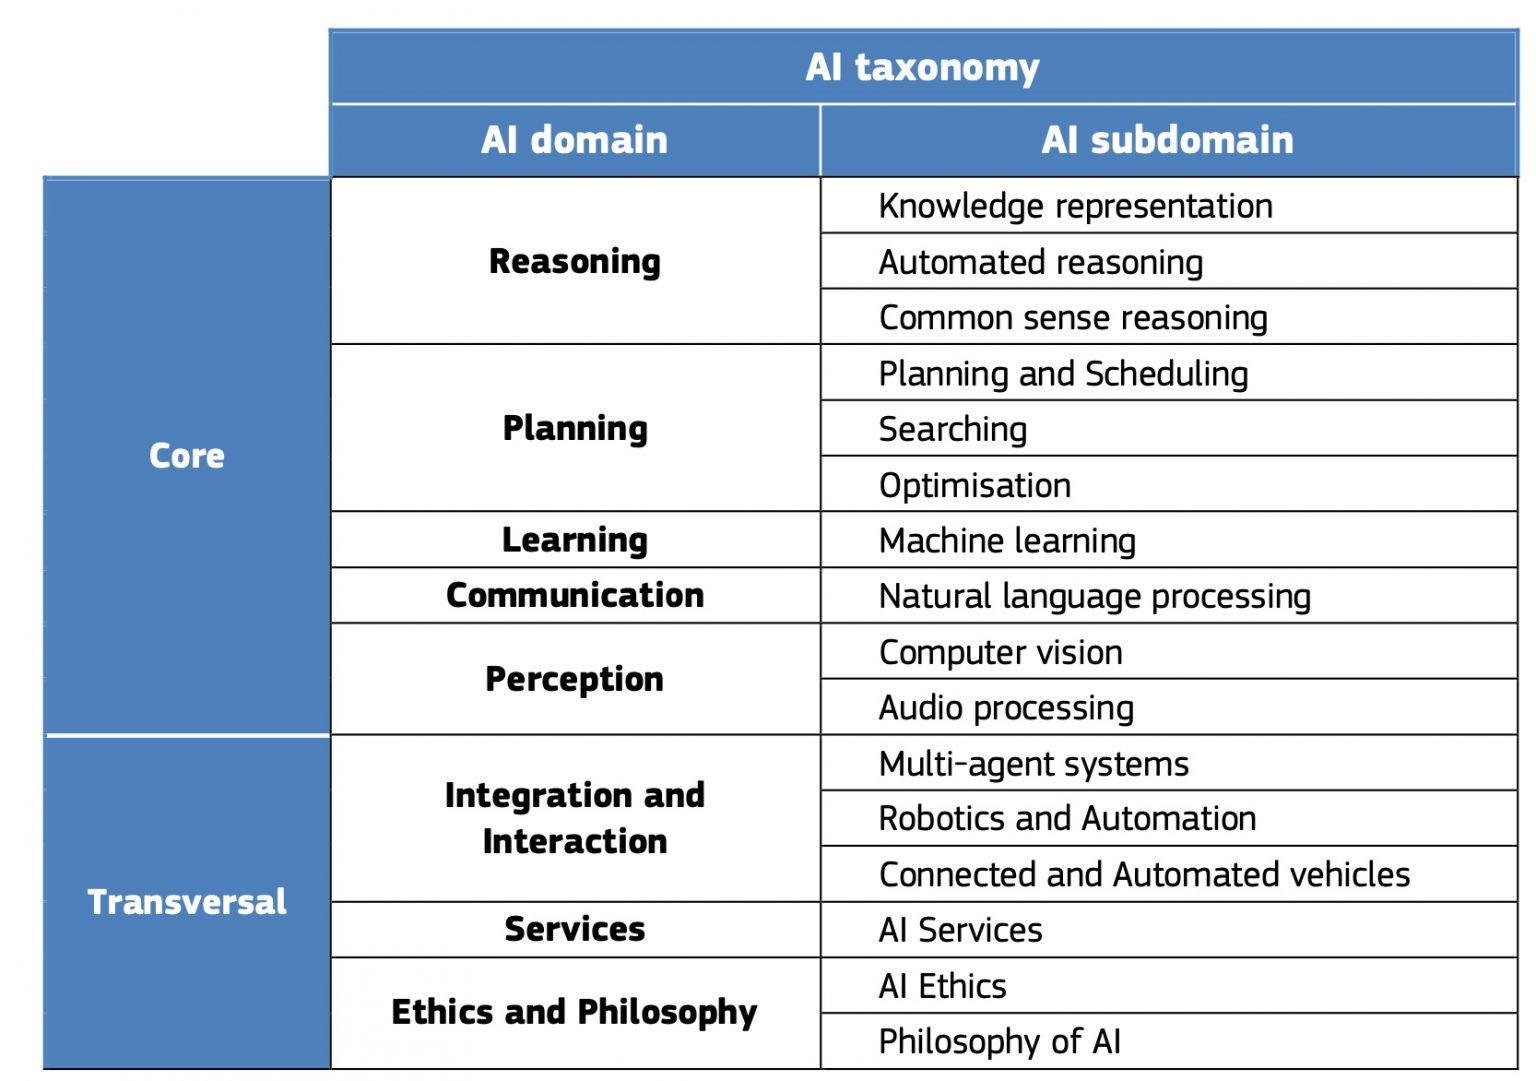
\includegraphics{img/taxonomia.jpg}
\end{adjustbox}
\caption{Taxonomía de la IA aplicada a la industria}
\label{fig:taxonomia-ia}
\end{figure}

Esta imagen presenta una \textbf{taxonomía de la Inteligencia Artificial (IA)}, organizada en dominios y subdominios, que abarca tanto aspectos \textbf{centrales (Core)} como \textbf{transversales (Transversal)} de la IA. Aquí te explico cada sección:

\subsection{Dominio Central (Core)}\label{dominio-central-core}
Estos son los fundamentos o los componentes clave de la IA, que abarcan desde cómo razona una máquina hasta cómo percibe e interactúa con el mundo.

\begin{enumerate}
\item \textbf{Reasoning (Razonamiento)}
  \begin{itemize}
    \item \textbf{Knowledge Representation}: Representación del conocimiento. Se refiere a cómo una máquina organiza y almacena la información de manera que pueda usarla para tomar decisiones o resolver problemas.
    \item \textbf{Automated Reasoning}: Razonamiento automatizado. La capacidad de la IA para derivar conclusiones y resolver problemas complejos basados en las reglas y el conocimiento almacenado.
    \item \textbf{Common Sense Reasoning}: Razonamiento de sentido común. La IA intenta razonar como lo haría una persona, utilizando conocimientos que los humanos damos por sentado, pero que las máquinas deben aprender o codificar.
  \end{itemize}

\item \textbf{Planning (Planificación)}
  \begin{itemize}
    \item \textbf{Planning and Scheduling}: Planificación y programación. La capacidad de la IA para organizar tareas o recursos en función de objetivos, optimizando tiempos y recursos.
    \item \textbf{Searching}: Búsqueda. IA encuentra soluciones a problemas o información relevante entre un conjunto de opciones.
    \item \textbf{Optimisation}: Optimización. Aquí la IA busca la mejor solución entre múltiples alternativas, ajustando variables para obtener el mejor rendimiento o eficiencia.
  \end{itemize}

\item \textbf{Learning (Aprendizaje)}
  \begin{itemize}
    \item \textbf{Machine Learning}: Aprendizaje automático. Esta es la capacidad de las máquinas para aprender a partir de datos sin ser programadas explícitamente para cada tarea. Es una de las áreas más destacadas y utilizadas en la IA actual.
  \end{itemize}

\item \textbf{Communication (Comunicación)}
  \begin{itemize}
    \item \textbf{Natural Language Processing}: Procesamiento del lenguaje natural. La IA comprende, interpreta y genera lenguaje humano, facilitando la interacción entre humanos y máquinas mediante el habla o el texto.
  \end{itemize}

\item \textbf{Perception (Percepción)}
  \begin{itemize}
    \item \textbf{Computer Vision}: Visión por computadora. La IA percibe el mundo visualmente, analizando imágenes o videos para detectar patrones, objetos o reconocer caras.
    \item \textbf{Audio Processing}: Procesamiento de audio. Similar a la visión por computadora, pero en este caso, la IA procesa y entiende sonidos, como la voz o música.
  \end{itemize}
\end{enumerate}

\subsection{Dominio Transversal}\label{dominio-transversal}

Estas áreas complementan los dominios centrales, ofreciendo integración, interacción y aspectos filosóficos o éticos.

\begin{enumerate}
\item \textbf{Integration and Interaction (Integración e Interacción)}
  \begin{itemize}
    \item \textbf{Multi-agent Systems}: Sistemas multiagente. Conjunto de IA que trabajan juntas, colaborando o compitiendo para resolver problemas más complejos.
    \item \textbf{Robotics and Automation}: Robótica y automatización. Integra la IA con robots y sistemas automatizados para realizar tareas físicas, como ensamblar productos en fábricas.
    \item \textbf{Connected and Automated Vehicles}: Vehículos conectados y automatizados. Implica el uso de IA para controlar vehículos autónomos y conectados que operan sin intervención humana.
  \end{itemize}

\item \textbf{Services (Servicios)}
  \begin{itemize}
    \item \textbf{AI Services}: Servicios de IA. Herramientas y plataformas basadas en IA que las empresas y personas pueden utilizar para resolver problemas o mejorar procesos (por ejemplo, asistentes virtuales, análisis predictivos).
  \end{itemize}

\item \textbf{Ethics and Philosophy (Ética y Filosofía)}
  \begin{itemize}
    \item \textbf{AI Ethics}: Ética de la IA. Se ocupa de las cuestiones éticas relacionadas con el uso y el desarrollo de la IA, como la privacidad, la equidad y el impacto social.
    \item \textbf{Philosophy of AI}: Filosofía de la IA. Reflexiones más profundas sobre el papel de la IA en la sociedad y qué significa para las máquinas tener inteligencia similar a la humana.
  \end{itemize}
\end{enumerate}

\subsection{Resumen}\label{resumen}

La taxonomía de la IA presentada en esta imagen divide los conceptos fundamentales en dominios que abarcan \textbf{razonamiento}, \textbf{planificación}, \textbf{aprendizaje}, \textbf{comunicación} y \textbf{percepción}. Estos conceptos son claves para entender cómo la IA interactúa y aprende del mundo. Los dominios transversales complementan estas capacidades con aspectos como la \textbf{integración}, los \textbf{servicios de IA} y las \textbf{cuestiones éticas}, que son fundamentales para asegurar un uso responsable y eficaz de la inteligencia artificial en el mundo real.


\section{IA Simbólica}\label{ia-simbolica}

La Inteligencia Artificial Simbólica es un enfoque de la IA que se basa en representar el conocimiento y el razonamiento a través de símbolos y reglas lógicas. En lugar de aprender a partir de datos, como ocurre en el Machine Learning, la IA simbólica funciona siguiendo un conjunto de instrucciones predefinidas para resolver problemas o tomar decisiones.

Por ejemplo, en una maquiladora donde se ensamblan componentes electrónicos, la IA simbólica puede controlar la temperatura de las máquinas o la calidad de los productos sin margen de error, gracias a sus reglas fijas. Este enfoque es ideal para tareas donde no hay mucha variabilidad, y se requiere cumplir con estrictos parámetros de producción.

Este enfoque es como una receta: todo está previamente determinado, y la máquina sigue los pasos sin desviarse. Un sistema de IA simbólica podría estar programado para diagnosticar fallos en una máquina si ciertas condiciones, como la temperatura o la vibración, exceden los límites establecidos. Cada condición está claramente definida, y la IA actúa según las reglas sin necesidad de adaptarse o aprender nuevas formas de solucionar el problema.

La IA Simbólica es particularmente útil en entornos donde los procesos son repetitivos o bien estructurados. Aunque no es flexible como el Machine Learning, la IA simbólica es extremadamente precisa y eficiente cuando se trata de ejecutar tareas que siguen un patrón fijo y bien entendido.

\subsection{Ejemplo: IA Simbólica con Receta de Cocina}\label{ejemplo-ia-simbolica}

\textbf{Imagina} que le das a un robot una receta detallada para hacer un pastel. Le das instrucciones específicas como:

\begin{enumerate}
    \item Mezcla 200 gramos de harina con 100 gramos de azúcar.
    \item Añade dos huevos y bate la mezcla por 5 minutos.
    \item Coloca la mezcla en el horno a 180°C durante 30 minutos.
\end{enumerate}

Este tipo de robot es un ejemplo de \textbf{IA Simbólica}, porque sigue un conjunto de reglas claras para completar la tarea. Cada paso está definido de manera precisa, y el robot simplemente sigue las instrucciones. Si la receta no cambia, el robot siempre hará el pastel de la misma manera, una y otra vez.

\subsection{Ejemplo: Machine Learning como Chef Aprendiz}\label{ejemplo-machine-learning}

Ahora, \textbf{imagina} que en lugar de seguir siempre la misma receta, tienes un robot que quiere convertirse en un chef experto. En lugar de seguir instrucciones precisas, este robot observa a diferentes cocineros haciendo pasteles y aprende de sus técnicas. Tal vez nota que algunos cocineros usan más azúcar, otros agregan ingredientes extra como vainilla, y algunos hornean el pastel por más tiempo dependiendo del tipo de horno. El robot comienza a \textbf{aprender} que, dependiendo de ciertos factores, puede ajustar la receta para hacer el mejor pastel posible.

Este es un ejemplo de \textbf{Machine Learning}, donde la IA no sigue reglas predefinidas, sino que aprende a partir de los datos que recopila. En lugar de seguir la misma receta siempre, el robot adapta la receta según los datos que ha recopilado.

\subsection{Comparando los Enfoques}\label{comparacion-enfoques}

\begin{itemize}
    \item \textbf{IA Simbólica}: Es como el robot que sigue una receta fija. Funciona bien en situaciones donde las reglas son claras y no cambian mucho. Esto es útil en procesos repetitivos como el ensamblaje en una maquila, donde los pasos son los mismos cada día.
    \item \textbf{Machine Learning}: Es como el chef aprendiz. En lugar de seguir reglas fijas, aprende y mejora con el tiempo a medida que recopila más información.
\end{itemize}

\subsection{Ejemplo: IA en el Control de Calidad}\label{ejemplo-control-calidad}

\textbf{Imagina} que en tu maquila produces miles de piezas cada día, y necesitas asegurarte de que todas cumplan con los estándares de calidad. En lugar de tener a una persona revisando cada pieza (lo cual puede ser lento y propenso a errores), podrías usar \textbf{IA Simbólica} o \textbf{Machine Learning}.

\begin{itemize}
    \item Con \textbf{IA Simbólica}, podrías programar una máquina para revisar cada pieza siguiendo reglas específicas. Por ejemplo: ``Si la pieza tiene más de 0.5 mm de desviación, recházala''. Esto es eficiente, pero solo funciona para detectar errores simples.
    \item Con \textbf{Machine Learning}, podrías entrenar una máquina para detectar patrones más complejos. El sistema podría aprender a reconocer qué tipo de defectos aparecen con mayor frecuencia y, con el tiempo, predecir dónde y cuándo es más probable que aparezcan defectos, ajustando la producción en consecuencia. Podría incluso aprender de nuevos datos para mejorar la precisión a lo largo del tiempo.
\end{itemize}

\subsection{Reflexión Final: Bajar la IA a lo Práctico}\label{reflexion-practica}

La IA, en su forma más simple, es una herramienta que ayuda a las máquinas a hacer tareas que normalmente haría un humano, pero con mayor precisión y eficiencia. No necesitas ser un experto para empezar a entender cómo puede mejorar tu maquila. Lo importante es reconocer que hay dos formas principales en que la IA puede ayudarte: \textbf{siguiendo reglas fijas (IA Simbólica)} o \textbf{aprendiendo de los datos (Machine Learning)}. Y aunque los conceptos técnicos puedan sonar complicados, los beneficios prácticos son claros: más eficiencia, menos errores, y una producción más ágil y adaptada a las necesidades del día a día.

\section{Perfil para Trabajar con IA Simbólica en una Maquiladora}\label{perfil-ia-simbolica}

Para implementar y gestionar la \textbf{IA Simbólica} en una maquiladora, se necesita un perfil multidisciplinario que combine habilidades técnicas con un profundo conocimiento de los procesos industriales. A continuación, te describo el perfil ideal para alguien que trabajará en la adopción y gestión de la IA simbólica en un entorno de producción.

\subsection{Conocimiento Técnico en Programación y Lógica}

Dado que la IA simbólica se basa en reglas predefinidas y condiciones lógicas, es crucial que el candidato tenga sólidos conocimientos de \textbf{programación} y \textbf{lógica de procesos}. Estos son algunos de los requisitos técnicos:

\begin{itemize}
    \item \textbf{Lenguajes de Programación}: Competencia en lenguajes de programación que permiten definir reglas y algoritmos, como \textbf{Python}, \textbf{C++}, o lenguajes específicos de automatización industrial (como \textbf{Ladder Logic} o \textbf{Structured Text} para PLCs).
    \item \textbf{Experiencia en Sistemas de Automatización}: Conocimiento de sistemas SCADA o PLC (Controladores Lógicos Programables) que se utilizan ampliamente en entornos industriales.
    \item \textbf{Manejo de Reglas Lógicas}: Habilidad para diseñar y gestionar reglas de ``si-entonces'' (if-then) y otros tipos de reglas lógicas que determinan el comportamiento de los sistemas de IA simbólica.
    \item \textbf{Diagramas de Flujo}: Capacidad para diseñar, interpretar y modificar diagramas de flujo que describen el funcionamiento del sistema de IA simbólica.
\end{itemize}

\subsection{Conocimiento en Procesos Industriales}

Es fundamental que la persona tenga un buen entendimiento de los procesos específicos de la \textbf{industria maquiladora}. Esto permitirá al profesional identificar las áreas donde la IA simbólica puede ser más útil y generar un mayor impacto en la eficiencia y automatización de procesos.

\begin{itemize}
    \item \textbf{Control de Calidad}: Comprender cómo funcionan los sistemas de control de calidad en la línea de producción y cómo la IA puede optimizar el proceso mediante reglas predefinidas para la detección de defectos.
    \item \textbf{Gestión de Inventarios}: Saber cómo operan los sistemas de inventario y cómo las reglas lógicas pueden automatizar las órdenes de compra y el reabastecimiento.
    \item \textbf{Mantenimiento de Máquinas}: Conocimiento sobre los ciclos de mantenimiento y cómo establecer reglas simbólicas para alertas y paradas preventivas.
\end{itemize}

\subsection{Habilidad para Diseñar Sistemas Basados en Reglas}

Una de las tareas más importantes de este perfil es diseñar y optimizar las reglas que seguirá la IA simbólica. Esto requiere una capacidad para crear reglas claras y efectivas que cubran todas las posibles condiciones y escenarios que pueden presentarse en la maquiladora.

\begin{itemize}
    \item \textbf{Diseño de Reglas Condicionales}: Capacidad para desarrollar un sistema de reglas eficiente, asegurándose de que todas las situaciones posibles estén cubiertas. Ejemplo: ``Si el nivel de vibración de una máquina supera el umbral X, entonces enviar una alerta.''
    \item \textbf{Optimización de Procesos}: Habilidad para analizar y optimizar procesos mediante la creación de flujos lógicos claros, reduciendo tiempos muertos y aumentando la eficiencia de la producción.
\end{itemize}

\subsection{Experiencia en Implementación de Soluciones de IA Simbólica}

El candidato debe tener experiencia práctica en la implementación de sistemas basados en IA simbólica, desde el diseño inicial hasta la puesta en marcha y ajuste de reglas en entornos reales de producción.

\begin{itemize}
    \item \textbf{Configuración e Integración}: Capacidad para configurar la IA simbólica en los sistemas existentes, integrando la tecnología con otras soluciones industriales como ERPs, SCADA, o sistemas de gestión de inventarios.
    \item \textbf{Pruebas y Validación}: Habilidad para realizar pruebas y validar que las reglas y condiciones están funcionando de acuerdo con lo esperado, ajustando según sea necesario para mejorar la precisión del sistema.
\end{itemize}

\section{Ejemplo Práctico: Sistema de Control de Inventario}\label{ejemplo-control-inventario}

Imagina que en tu maquiladora manejas grandes cantidades de inventario y necesitas automatizar el proceso de reabastecimiento. Tradicionalmente, un encargado del almacén revisa manualmente los niveles de stock y crea órdenes de compra cuando se está quedando sin material. Este proceso manual puede ser ineficiente, propenso a errores y muy dependiente de una sola persona.

Al implementar un sistema basado en \textbf{IA Simbólica}, puedes automatizar este proceso completamente, eliminando la necesidad de revisiones manuales y reduciendo la dependencia del personal para mantener los niveles de stock óptimos. El sistema analizaría continuamente los niveles de inventario y generaría órdenes de compra automáticamente cuando sea necesario.

\subsection{Dataset de Ejemplo para Mantenimiento Predictivo}\label{dataset-mantenimiento-predictivo}

Además de optimizar el inventario, la IA también puede utilizarse para el mantenimiento predictivo de las máquinas. A continuación, se muestra un ejemplo de un dataset que podría usarse para entrenar un modelo de Machine Learning que prediga cuándo es probable que una máquina falle o necesite mantenimiento:

\begin{table}[htbp]
\centering
\begin{tabular}{|c|c|c|c|c|}
\hline
ID Máquina & Temperatura & Horas de Operación & Tipo de Máquina & Mantenimiento Urgente \\
\hline
1 & 85°C & 200 & Soldadora & Sí \\
2 & 70°C & 300 & Ensambladora & No \\
3 & 90°C & 180 & Cortadora & Sí \\
\hline
\end{tabular}
\caption{Ejemplo de dataset de mantenimiento predictivo en maquiladoras}
\label{tab:mantenimiento-predictivo}
\end{table}

Este dataset puede ser usado para entrenar un modelo de Machine Learning que prediga si una máquina va a necesitar mantenimiento en el futuro. El modelo analizaría las variables (temperatura, horas de operación, tipo de máquina) para predecir cuándo será necesario el mantenimiento, permitiendo que las intervenciones sean más proactivas en lugar de reactivas.

\subsection{Diagrama de Flujo para IA Simbólica}\label{diagrama-flujo}

Un diagrama de flujo es una representación gráfica de un proceso. En el caso de la IA simbólica, se puede utilizar para ilustrar cómo las reglas lógicas guían el comportamiento del sistema. Estas reglas definen un conjunto claro de condiciones, y el sistema actúa automáticamente dependiendo de si se cumplen o no.

\begin{figure}[H]
\centering
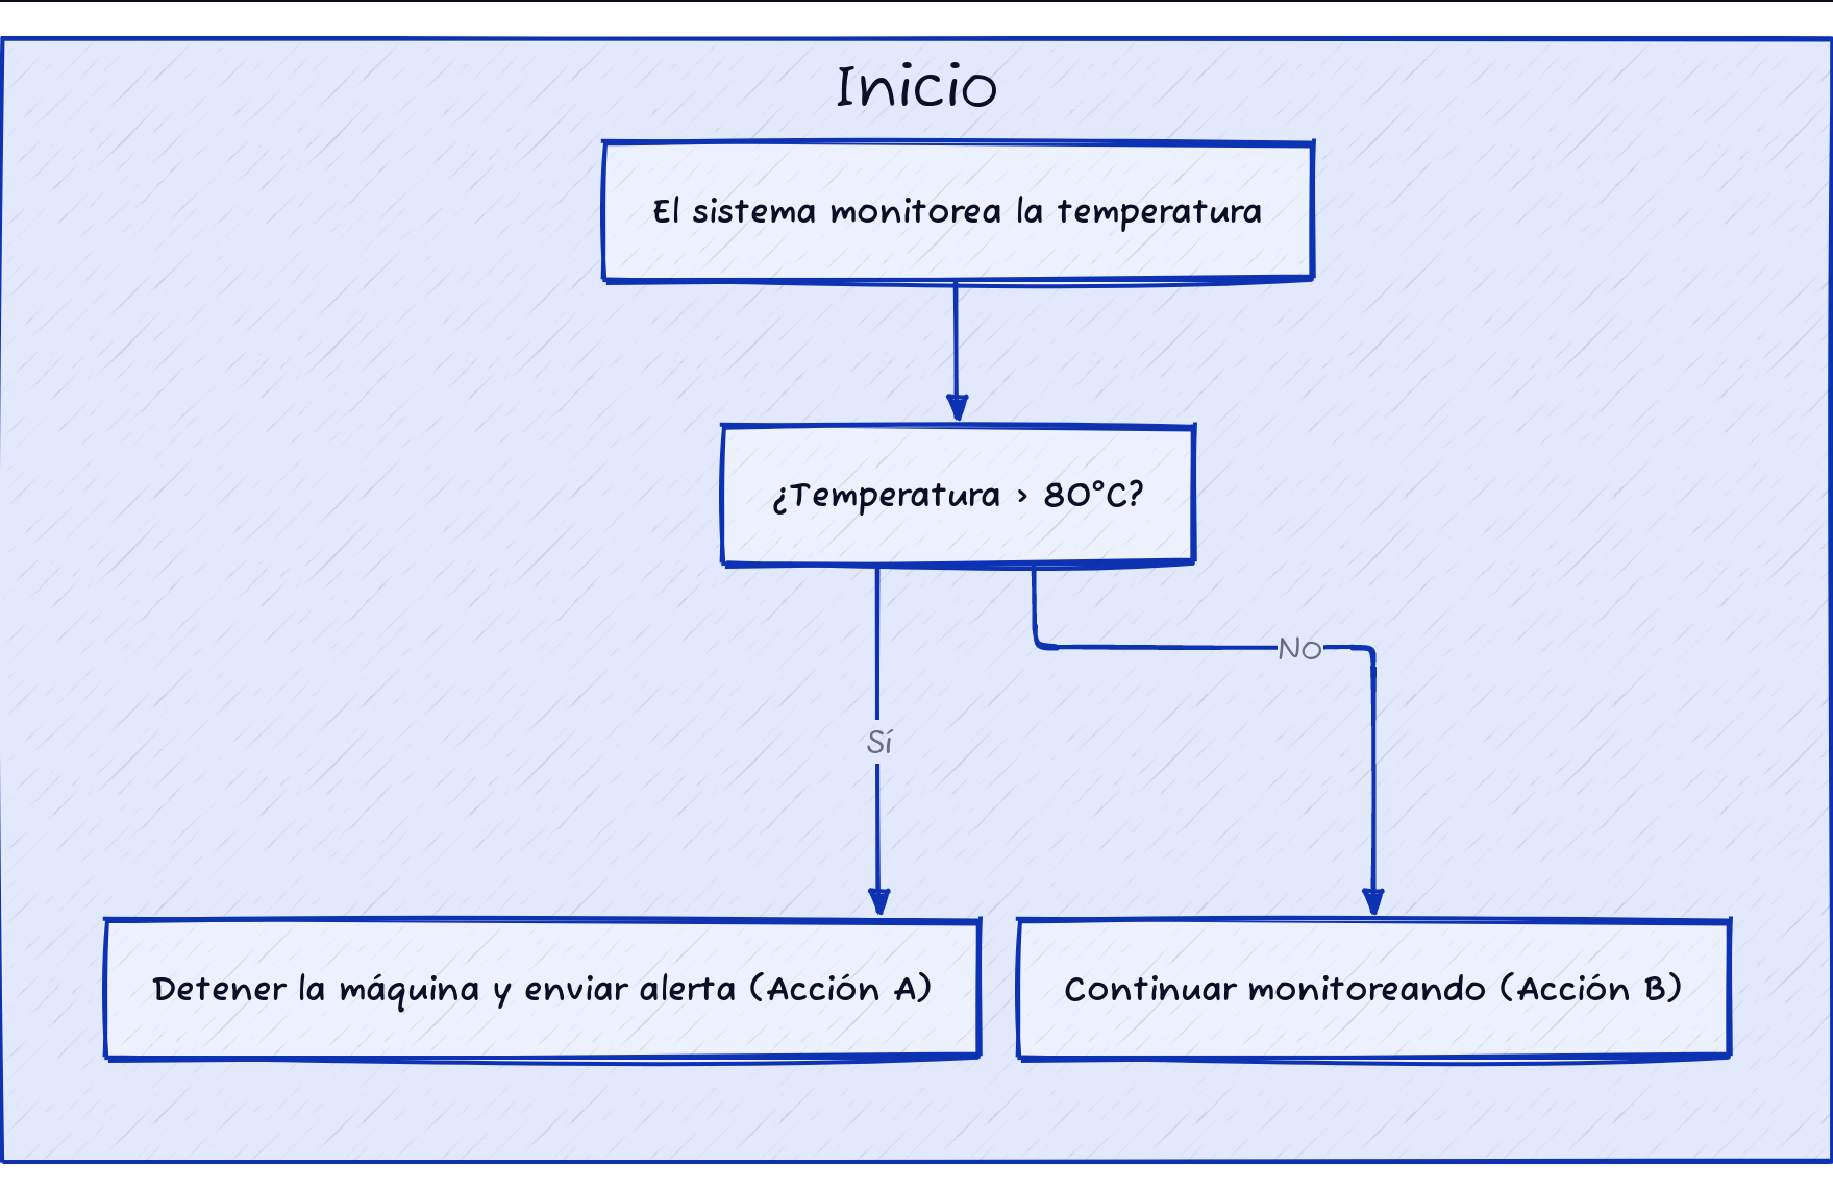
\includegraphics[h!,scale=0.5]{pdfs/diagram-1.pdf} 
\caption{Diagrama de flujo para IA simbólica en un sistema de inventario}
\label{fig:diagrama-flujo}
\end{figure}

En este flujo, cada decisión está basada en una condición clara que lleva a una acción específica. Esto es exactamente cómo funciona la IA simbólica: sigue reglas predefinidas sin necesidad de aprender o ajustarse con el tiempo. Por ejemplo:

\begin{itemize}
    \item \textbf{Condición 1:} Si el nivel de stock de un producto es menor a 50 unidades, enviar una alerta.
    \item \textbf{Condición 2:} Si el nivel de stock es menor a 10 unidades, generar automáticamente una orden de compra.
\end{itemize}

Este tipo de lógica reduce significativamente la intervención manual, permitiendo que el sistema mantenga el inventario de manera eficiente y asegurando que nunca haya falta de material para la producción.

\subsection{Implementación de un Sistema de Control de Inventario Basado en IA Simbólica}\label{implementacion-control-inventario}

Para implementar un sistema de control de inventario basado en \textbf{IA Simbólica}, los siguientes pasos serían esenciales:

\begin{enumerate}
    \item \textbf{Identificación de Variables Críticas:} El primer paso es identificar qué variables son clave para el proceso de control de inventario. Esto puede incluir el nivel de stock actual, la demanda histórica del producto, y el tiempo de reabastecimiento de los proveedores.
    
    \item \textbf{Definición de Reglas de Negocio:} Una vez identificadas las variables críticas, se deben definir las reglas de negocio que el sistema seguirá. Por ejemplo, \textit{"Si el nivel de stock de un producto es menor a 50 unidades, generar una alerta"}.
    
    \item \textbf{Automatización de Decisiones:} El sistema debe ser capaz de tomar decisiones automáticas basadas en estas reglas de negocio. Esto incluye la generación automática de órdenes de compra cuando los niveles de stock caigan por debajo de un umbral predefinido.
    
    \item \textbf{Monitoreo y Ajuste del Sistema:} Una vez que el sistema esté en funcionamiento, es importante monitorear su desempeño y realizar ajustes según sea necesario. Esto puede incluir la modificación de las reglas o la incorporación de nuevas variables.
\end{enumerate}

El beneficio de este tipo de sistema es que es extremadamente preciso y elimina el riesgo de errores humanos. Además, reduce la necesidad de intervención manual en procesos que de otro modo serían tediosos y propensos a errores.

\subsection{Diagrama de Flujo Extendido para IA Simbólica}\label{diagrama-flujo-extendido}

En un sistema más complejo, la IA simbólica puede manejar múltiples condiciones y tomar decisiones en función de diversos factores, como se muestra en el siguiente diagrama de flujo:

\begin{figure}[H]
\centering
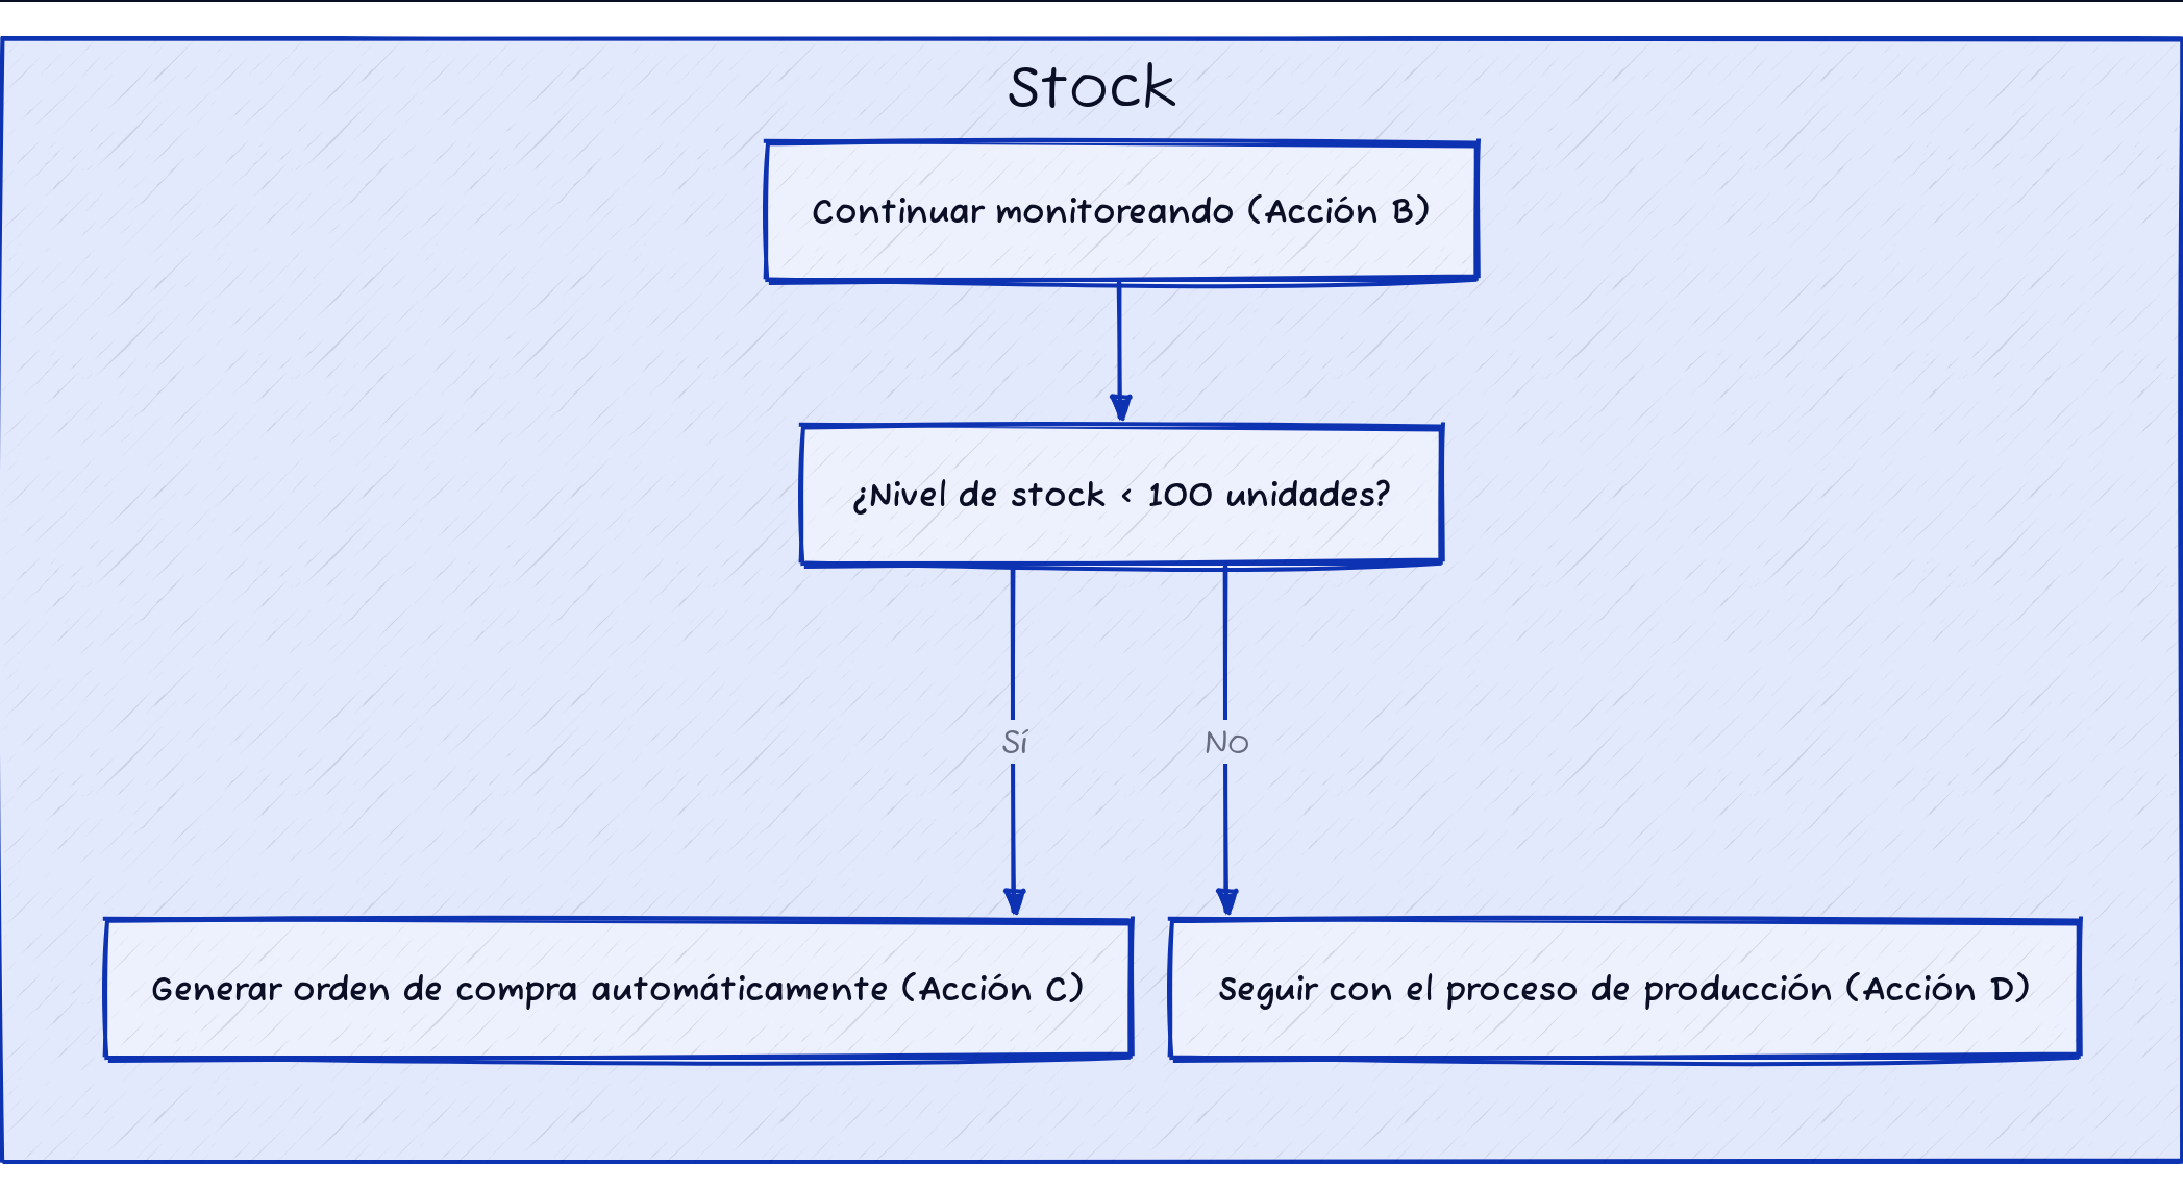
\includegraphics[h!,scale=0.5]{pdfs/diagram-2.pdf} 
\caption{Diagrama de flujo extendido para IA simbólica en un sistema de inventario}
\label{fig:diagrama-flujo-extendido}
\end{figure}

Este diagrama de flujo muestra un sistema de control de inventario más sofisticado que considera no solo los niveles de stock, sino también factores como el tiempo de entrega de los proveedores, la variabilidad de la demanda y los tiempos de producción.

\subsection{Conclusión: Primer Paso hacia la Automatización Inteligente}\label{conclusion}

La \textbf{IA Simbólica} es un paso esencial para que tu maquila avance hacia la automatización. Al establecer reglas claras y estructuradas, respaldadas por diagramas de flujo, puedes asegurar que todos los procesos se realicen de manera eficiente, sin depender de una sola persona o archivo.

Además, los sistemas basados en IA simbólica son ideales para procesos bien definidos y repetitivos, como el control de inventario y el mantenimiento preventivo. Si tu maquiladora aún depende de procesos manuales para gestionar el inventario o el mantenimiento, implementar IA simbólica te permitirá mejorar significativamente la eficiencia y reducir costos operativos.

\subsection{IA Simbólica: El Futuro del Control de Inventario}\label{futuro-ia-simbolica}

Al considerar el futuro del control de inventario en una maquiladora, la IA simbólica es solo el primer paso hacia una mayor automatización. Conforme avanza la tecnología, será posible integrar \textbf{Machine Learning} y \textbf{Big Data} para hacer que los sistemas no solo sigan reglas predefinidas, sino que también aprendan de los datos históricos y ajusten las reglas dinámicamente para optimizar aún más la eficiencia.

Por ejemplo, un sistema que combine IA simbólica con Machine Learning podría ajustar automáticamente los niveles mínimos de stock en función de la demanda estacional o las variaciones en los tiempos de entrega de los proveedores, optimizando continuamente el inventario sin necesidad de intervención humana.

\subsection{Implementación Práctica en el Contexto Actual}\label{implementacion-practica}

Hoy en día, muchas maquiladoras ya han comenzado a implementar sistemas basados en IA simbólica para la gestión del inventario, lo que ha reducido significativamente los tiempos de inactividad debido a la falta de materiales. Además, la reducción de errores humanos ha permitido a estas empresas operar de manera más eficiente y aumentar su productividad.

La implementación de sistemas de IA simbólica no requiere una infraestructura compleja. En muchos casos, se pueden integrar con los sistemas de ERP (Planificación de Recursos Empresariales) existentes, lo que facilita la transición hacia un modelo de producción más automatizado. 

Finalmente, una maquiladora que adopte IA simbólica y otras tecnologías relacionadas estará mejor preparada para enfrentar los retos de la industria 4.0, mejorando tanto su competitividad como su capacidad para responder rápidamente a las demandas del mercado.


%%%%%%%%%%%%%%%%%%%%%%%%%%%%%%%%%%%%%%%%%%%%%%%%%%%%%%%%%%%%%%%%%%%%%%%%%%%%%%%%%%%%%%%%%%%%%%
\section{Aplicaciones de Machine Learning en la Maquiladora}\label{aplicaciones-de-machine-learning-en-la-maquiladora}

\subsection{\textbf{Introducción a Machine Learning (ML)}}\label{introduccion-a-machine-learning-ml}

El \textbf{Machine Learning} es una herramienta clave en el avance tecnológico de las maquiladoras. Aunque suena como un concepto complicado, en realidad es más sencillo de lo que parece: se trata de enseñar a las máquinas a \textbf{aprender} de los datos, tal como nosotros aprendemos de la experiencia. En lugar de programar una máquina para que haga exactamente lo que queremos (como en los sistemas tradicionales), \textbf{Machine Learning (ML)} permite que las máquinas identifiquen patrones, hagan predicciones y tomen decisiones basadas en esos datos.

Entonces, \textbf{¿por qué esto es importante para una maquiladora?} Porque la IA y el Machine Learning pueden ayudar a reducir errores, optimizar la producción, mejorar la calidad y anticipar problemas antes de que ocurran. Si tu línea de producción tiene un historial de fallas que cuesta tiempo y dinero, ¿no sería genial que una máquina te avisara antes de que suceda para que pudieras arreglarlo de antemano?

\begin{figure}[H]
\centering
\begin{adjustbox}{width=\textwidth}
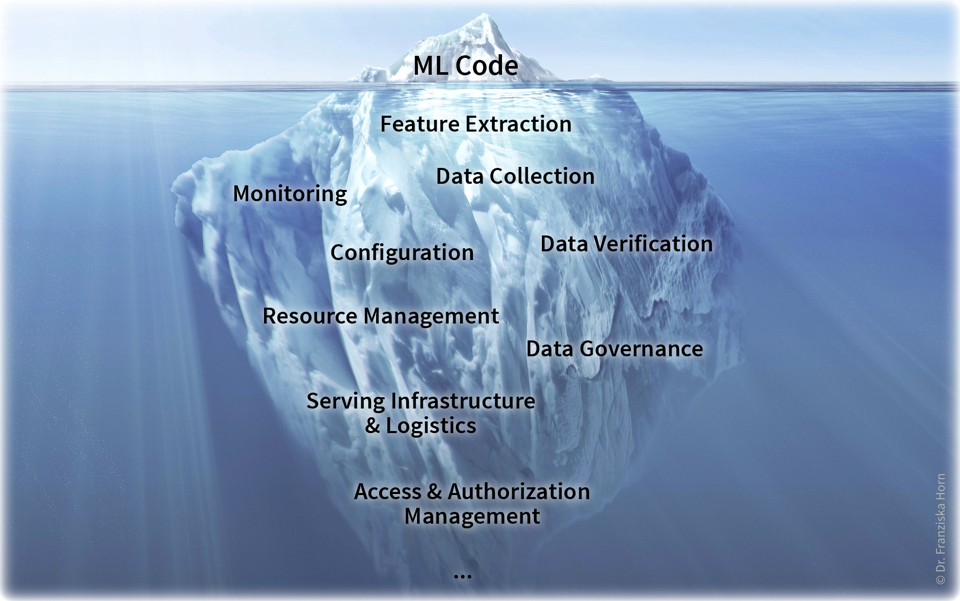
\includegraphics{img/imagen_186.jpg}
\end{adjustbox}
\caption{Meme sobre Machine Learning en la maquila}
\end{figure}

\section{\textbf{¿Qué es Machine Learning?}}\label{que-es-machine-learning}

El \textbf{Machine Learning} se basa en la idea de que una máquina puede aprender a hacer algo (como predecir fallas o mejorar un proceso) simplemente dándole acceso a muchos datos sobre ese algo. \textbf{Es como enseñar a alguien a resolver un problema dándole ejemplos de cómo se ha resuelto ese problema antes.}

Imagina que tienes datos sobre la producción de una máquina: las horas que opera, las temperaturas que alcanza, la cantidad de piezas que fabrica, etc. Si cada vez que la máquina fallaba también anotabas estas mismas características, podrías darle esos datos a un modelo de Machine Learning, y este aprendería a identificar las condiciones que llevan a una falla. \textbf{Básicamente, se trata de darle a la máquina un ``historial'' de lo que ha pasado, para que pueda predecir lo que pasará en el futuro}.

En resumen: \textbf{Machine Learning} es el arte de hacer que las máquinas aprendan de los datos, para que puedan tomar decisiones o hacer predicciones sin que les digas exactamente qué hacer en cada caso.

\begin{figure}[H]
\centering
\begin{adjustbox}{width=\textwidth}
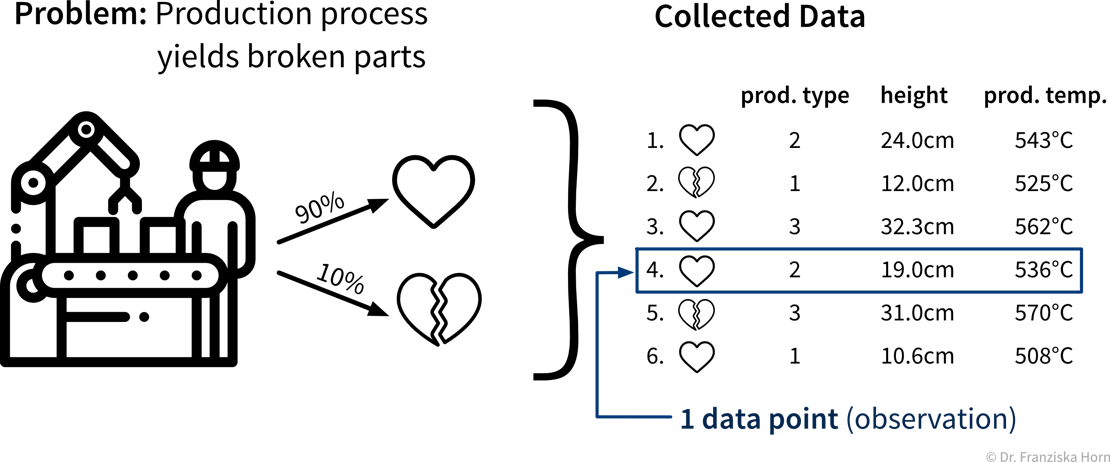
\includegraphics{img/imagen_32.jpg}
\end{adjustbox}
\caption{Meme sobre la predicción en Machine Learning}
\end{figure}

\subsubsection{\textbf{Aprendizaje Supervisado vs No Supervisado}}\label{aprendizaje-supervisado-vs-no-supervisado}

Existen dos tipos principales de Machine Learning, y entender la diferencia entre ellos te ayudará a identificar cuál es más útil en tu maquila.

\subsubsection{\textbf{Aprendizaje Supervisado}}\label{aprendizaje-supervisado}

El \textbf{aprendizaje supervisado} es como enseñarle a alguien a hacer algo mostrándole los ejemplos correctos y las respuestas. Le das a la máquina un conjunto de datos donde ya sabes lo que pasa (el resultado), y la máquina aprende a predecir ese resultado cuando vea datos nuevos.

\textbf{Ejemplo sencillo en la maquila}: Supón que tienes los datos de las máquinas en tu línea de producción y sabes qué condiciones llevaron a una falla (como vibraciones anormales o temperaturas extremas). Puedes entrenar a un modelo de Machine Learning para que, cuando vea esas mismas condiciones en una máquina en funcionamiento, te avise de que algo está mal antes de que ocurra una avería.

Este tipo de ML funciona muy bien cuando ya tienes información sobre lo que ha ocurrido y quieres predecir lo que sucederá en situaciones similares en el futuro.

\subsubsection{\textbf{Aprendizaje No Supervisado}}\label{aprendizaje-no-supervisado}

Por otro lado, el \textbf{aprendizaje no supervisado} es un poco más libre: es como darle un montón de información a la máquina y dejarla que descubra patrones por sí sola. No le dices qué debe buscar, simplemente la máquina agrupa los datos o encuentra similitudes entre ellos.

\textbf{Ejemplo sencillo en la maquila}: Digamos que tienes muchos datos sobre el rendimiento de tus máquinas, pero no sabes qué está afectando a la producción. Con el aprendizaje no supervisado, puedes descubrir patrones en los datos, como que ciertas máquinas siempre rinden menos a ciertas horas del día o cuando operan junto a otras máquinas específicas. La IA encontrará esos patrones, lo que te permitirá hacer ajustes en la producción que de otro modo no habrías notado.

\subsubsection{\textbf{El papel de ML en la maquila: ¿Por qué es importante?}}\label{el-papel-de-ml-en-la-maquila-por-que-es-importante}

Machine Learning puede transformar radicalmente la manera en que operas en la maquiladora. \textbf{¿Por qué?} Porque la IA no solo se trata de automatizar, sino de hacer más inteligentes las decisiones que tomas día a día.

\textbf{Imagina esto}: Tienes una línea de producción donde algunas máquinas fallan de vez en cuando. Esto significa paradas inesperadas, retrasos, y por supuesto, costos adicionales. Pero ¿qué pasaría si pudieras predecir cuándo esas máquinas van a fallar y hacer el mantenimiento antes de que ocurra la avería? Esto es lo que Machine Learning puede hacer por ti. Es como tener un ``sexto sentido'' en la producción.

Además, no solo hablamos de evitar fallas: Machine Learning puede ayudarte a ajustar el inventario de manera eficiente, prever la demanda, mejorar la calidad de los productos, y hasta optimizar la logística dentro de la planta. En resumen, \textbf{es una herramienta para ser más competitivo en un mercado que no para de moverse}.

\subsection{\textbf{Tipos de Machine Learning en la Maquila}}\label{tipos-de-machine-learning-en-la-maquila}

Ahora que ya tienes una idea básica de lo que es Machine Learning y por qué es tan relevante en la maquiladora, vamos a profundizar un poco más en los tipos de ML que puedes utilizar en tu planta. Dependiendo del tipo de problema que enfrentes, puedes elegir entre \textbf{aprendizaje supervisado} o \textbf{no supervisado}, e incluso otros enfoques como el \textbf{aprendizaje por refuerzo}.

\begin{figure}[H]
\centering
\begin{adjustbox}{width=\textwidth}
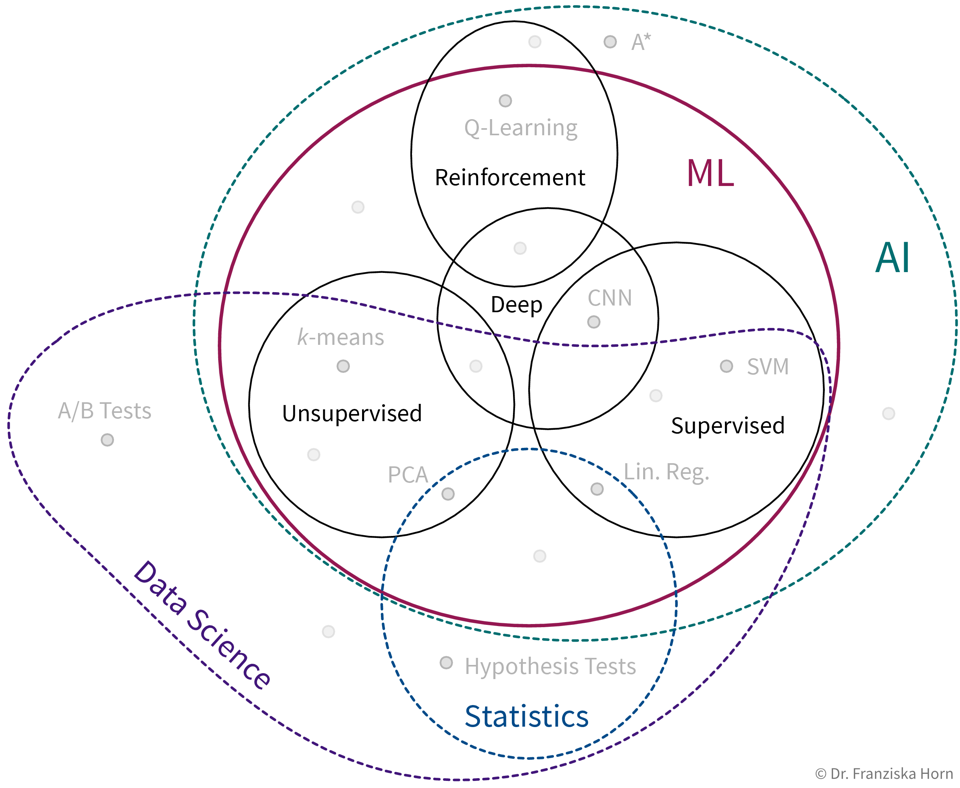
\includegraphics{img/imagen_21.jpg}
\end{adjustbox}
\caption{Meme sobre la importancia de elegir el tipo de Machine Learning}
\end{figure}

\subsubsection{\textbf{Aprendizaje Supervisado}}\label{aprendizaje-supervisado-1}

En el \textbf{aprendizaje supervisado}, el sistema aprende de datos que ya incluyen tanto las características (por ejemplo, temperatura de la máquina, tiempo de operación, etc.) como los resultados correctos (por ejemplo, si la máquina falló o no). Este tipo de aprendizaje es ideal cuando ya tienes un montón de información de tus procesos y quieres usarla para predecir futuros eventos.

\textbf{Ejemplo práctico}: Si sabes que ciertas condiciones en una máquina han llevado a su falla en el pasado, puedes entrenar un modelo de aprendizaje supervisado que prediga cuándo una máquina fallará de nuevo basándose en esas mismas condiciones. Esto es útil para el \textbf{mantenimiento predictivo}, que puede ahorrarte mucho tiempo y dinero.

\subsubsection{\textbf{Aprendizaje No Supervisado}}\label{aprendizaje-no-supervisado-1}

El \textbf{aprendizaje no supervisado} es como darle a la máquina una pila de datos y decirle ``¡descubre algo interesante!''. No le damos las respuestas de antemano, sino que la máquina encuentra patrones por su cuenta.

\textbf{Ejemplo práctico}: Puedes usar aprendizaje no supervisado para analizar datos de producción y descubrir relaciones que no habías visto antes. Por ejemplo, podrías descubrir que ciertas combinaciones de máquinas tienden a producir más errores en ciertos momentos del día. Este tipo de información es oro puro para optimizar la producción, ya que te permite tomar decisiones informadas basadas en lo que los datos te dicen, no en suposiciones.

\subsection{Conceptos Clave para Entender Machine Learning}\label{conceptos-clave-para-entender-machine-learning}

Para implementar \textbf{Machine Learning (ML)} de manera efectiva en una maquiladora, es fundamental comprender algunos conceptos clave que forman la base del aprendizaje automático. Estos términos te ayudarán a abordar los desafíos técnicos y a tomar decisiones más inteligentes a medida que avances en tu proceso de transformación digital.

\subsubsection{\textbf{Dataset: La Base de Todo}}\label{dataset-la-base-de-todo}

Un \textbf{dataset} es el conjunto de datos que alimenta al modelo de Machine Learning. \textbf{Piensa en el dataset como si fuera la materia prima de una maquiladora}, donde los datos son las piezas que la IA utiliza para aprender. Sin un buen dataset, el modelo no puede funcionar correctamente.

\textbf{Ejemplo en la maquila}: Supongamos que tienes datos históricos sobre las temperaturas de las máquinas, el tiempo que han estado operativas, el número de piezas que han producido y cuándo fallaron. Ese conjunto de datos es el ``dataset'' que alimentará tu modelo para que pueda aprender a predecir cuándo fallará una máquina en el futuro.

\subsubsection{\textbf{Variables Dependientes e Independientes}}\label{variables-dependientes-e-independientes}

En Machine Learning, las \textbf{variables} son los elementos de los datos que influyen en los resultados. Hay dos tipos de variables que debes conocer:

\begin{itemize}
    \item \textbf{Variables Independientes}: Son las entradas que proporcionan la información al modelo. Son como las características que describen un producto en una maquiladora. Por ejemplo, la temperatura de una máquina, la velocidad de producción o el número de horas trabajadas.
    \item \textbf{Variable Dependiente}: Es la salida o el resultado que estamos intentando predecir. Es lo que queremos que la máquina aprenda a identificar o calcular. En una maquiladora, la variable dependiente podría ser si una máquina va a fallar o no, o la cantidad de piezas defectuosas que produce una línea de producción.
\end{itemize}

\subsubsection{\textbf{Feature Engineering: La Clave del Éxito}}\label{feature-engineering-la-clave-del-exito}

El \textbf{feature engineering} es el proceso de elegir, transformar y crear las características (variables) que mejoran el rendimiento de un modelo de Machine Learning. Este paso es esencial porque no todas las variables son igual de útiles. Algunas variables pueden ser irrelevantes, mientras que otras pueden tener un impacto significativo en los resultados.

\subsubsection{\textbf{Preprocesamiento de Datos: Limpiando los Datos}}\label{preprocesamiento-de-datos-limpiando-los-datos}

El \textbf{preprocesamiento de datos} es uno de los pasos más importantes para que un modelo de Machine Learning funcione correctamente. Limpiarlos y prepararlos adecuadamente te permite sacar el máximo provecho de tu modelo de Machine Learning.

\subsection{\textbf{Ventajas del Machine Learning en la Maquiladora}}\label{ventajas-del-machine-learning-en-la-maquiladora}

El \textbf{Machine Learning} ofrece muchas ventajas para una maquiladora, desde la reducción de costos hasta la mejora en la eficiencia de los procesos. Aquí te detallamos las principales razones por las que integrar ML en tu maquila puede marcar la diferencia:

\subsubsection{\textbf{Rapidez en la Toma de Decisiones}}\label{rapidez-en-la-toma-de-decisiones}

Una de las mayores ventajas del Machine Learning es la \textbf{velocidad} con la que puede analizar grandes cantidades de datos y ofrecer resultados. Esto es especialmente útil en una maquiladora, donde la rapidez en la toma de decisiones puede marcar la diferencia entre cumplir con un pedido o retrasarse.

\subsubsection{\textbf{Facilidad de Uso y Sencillez}}\label{facilidad-de-uso-y-sencillez}

Hoy en día, las herramientas de Machine Learning son cada vez más accesibles, y muchas de ellas ofrecen interfaces simples que no requieren conocimientos avanzados en programación. Incluso si tu equipo no tiene experiencia con IA, \textbf{plataformas como AWS, Azure y Google Cloud} te permiten implementar modelos de manera sencilla y escalable.

\subsubsection{\textbf{Auditoría y Transparencia}}\label{auditoria-y-transparencia}

Otra ventaja clave es que \textbf{los modelos de Machine Learning pueden ser auditados}. Esto significa que puedes rastrear y verificar cómo el modelo llegó a una decisión o predicción, lo que es muy importante en industrias reguladas como la manufactura.

\subsection{\textbf{Desventajas del Machine Learning en la Maquiladora}}\label{desventajas-del-machine-learning-en-la-maquiladora}

Aunque \textbf{Machine Learning} tiene muchas ventajas, no es una solución mágica. Implementarlo también tiene desafíos y posibles desventajas que debes tener en cuenta.

\subsubsection{\textbf{Costo de Implementación}}\label{costo-de-implementacion}

A pesar de las ventajas a largo plazo, el costo inicial de implementar ML puede ser alto, especialmente si tu maquiladora no tiene ya la infraestructura necesaria.

\subsubsection{\textbf{Dudas Técnicas}}\label{dudas-tecnicas}

El éxito de un sistema de Machine Learning depende mucho de la calidad de los datos y del personal capacitado que pueda supervisar y ajustar los modelos.

\subsubsection{\textbf{Complejidad en el Análisis de Datos}}\label{complejidad-en-el-analisis-de-datos}

El análisis de datos en Machine Learning no es una tarea sencilla. Requiere tiempo y experiencia para preparar correctamente los datos, seleccionar las variables adecuadas y ajustar los modelos.

\subsection{\textbf{Conclusión de las Ventajas y Desventajas}}\label{conclusion-de-las-ventajas-y-desventajas}

En resumen, el \textbf{Machine Learning} tiene el potencial de revolucionar la maquiladora, optimizando procesos, reduciendo costos y mejorando la calidad de los productos. Sin embargo, la implementación tiene desafíos que deben considerarse cuidadosamente.

\subsection{\textbf{Referencias ML}}\label{referencias-ml}

\begin{enumerate}
    \item Russell, S. \& Norvig, P. \emph{Artificial Intelligence: A Modern Approach} (4th ed.). Prentice Hall, 2020.
    \item Goodfellow, I., Bengio, Y. \& Courville, A. \emph{Deep Learning}. MIT Press, 2016.
    \item Hastie, T., Tibshirani, R. \& Friedman, J. \emph{The Elements of Statistical Learning: Data Mining, Inference, and Prediction} (2nd ed.). Springer, 2009.
    \item Géron, A. \emph{Hands-On Machine Learning with Scikit-Learn, Keras, and TensorFlow} (2nd ed.). O'Reilly Media, 2019.
    \item Murphy, K. P. \emph{Machine Learning: A Probabilistic Perspective}. MIT Press, 2012.
    \item Bishop, C. M. \emph{Pattern Recognition and Machine Learning}. Springer, 2006.
\end{enumerate}


%$$$$$$$$$$$$$$$$$$$$
\section{¿Qué es el NLP?}\label{que-es-la-nlp}
El \textbf{procesamiento de lenguaje natural} (NLP, por sus siglas en inglés) es una tecnología de \textbf{machine learning} que permite a las computadoras interpretar, manipular y comprender el lenguaje humano. Gracias al NLP, las máquinas pueden interactuar con las personas utilizando lenguaje cotidiano de manera eficaz. Esto incluye tareas como el análisis de texto, la traducción automática, y la generación de respuestas a preguntas en lenguaje natural.

\begin{tikzpicture}[node distance=2cm]
    % Input (Entrada) con color
    \node (input) [draw, rectangle, fill=cyan!30, text width=6cm, align=left, rounded corners] 
    {Texto en lenguaje natural \\ \textbf{Ejemplo:} ``¿Cuántas unidades se produjeron hoy?''};
    
    % Procesamiento NLP con color
    \node (process) [below=of input, draw, rectangle, fill=yellow!30, text width=6cm, align=left, rounded corners] 
    {Procesamiento NLP \\ \textbf{Descripción:} El sistema descompone la frase, identifica palabras clave como ``unidades'' y ``hoy'', y analiza el contexto.};
    
    % Output (Salida) con color
    \node (output) [below=of process, draw, rectangle, fill=green!30, text width=6cm, align=left, rounded corners] 
    {Respuesta generada \\ \textbf{Ejemplo:} ``Se produjeron 500 unidades''};
    
    % Flechas de conexión con color
    \draw[->, thick, blue] (input) -- (process);
    \draw[->, thick, blue] (process) -- (output);
    
    % Descripción adicional debajo del diagrama
    \node at (-3, -11) [text width=15cm, align=center] 
    {Este diagrama muestra cómo funciona el procesamiento de lenguaje natural (NLP): el usuario introduce una pregunta en lenguaje natural (entrada), el sistema NLP la procesa, descomponiendo la frase e identificando el contexto, y luego genera una respuesta adecuada (salida).};
\end{tikzpicture}

\section{API: Interfaz de Programación de Aplicaciones}\label{api}
Una API (Interfaz de Programación de Aplicaciones) es un conjunto de reglas y especificaciones que facilita la comunicación e intercambio de datos entre distintas aplicaciones de software. Las APIs actúan como puentes digitales, permitiendo que diferentes tecnologías trabajen juntas sin problemas. Esto es esencial en un entorno moderno donde las aplicaciones y sistemas deben integrarse para ofrecer soluciones completas.

\subsection{Ventajas de las APIs}
Las APIs han revolucionado la forma en que las aplicaciones de software interactúan entre sí. Algunas de sus principales ventajas son:

\begin{itemize}
    \item \textbf{Reducción de costos y complejidad:} Permiten integrar servicios externos en lugar de desarrollar todo desde cero, lo que reduce tiempo, esfuerzo y costos de desarrollo.
    \item \textbf{Impulso a la innovación:} Los desarrolladores pueden aprovechar APIs existentes para acelerar el desarrollo de nuevas soluciones, lo que fomenta la creación rápida de productos innovadores.
    \item \textbf{Mejora de la experiencia de usuario:} APIs bien integradas permiten experiencias más completas y personalizadas al conectar diversas aplicaciones.
\end{itemize}

\subsection{Ejemplo Práctico}
Supongamos que estás desarrollando una aplicación financiera. En lugar de construir un sistema desde cero para manejar transacciones de criptomonedas, puedes utilizar la API de un servicio como \textbf{Gemini}. A través de esta API puedes realizar varias acciones, tales como:

\begin{itemize}
    \item Consultar precios de criptomonedas en tiempo real.
    \item Ejecutar órdenes de compra y venta.
    \item Realizar análisis de mercado en base a los datos obtenidos.
\end{itemize}

\section{La Nueva Era de la IA Generativa}\label{la-nueva-era-ia-generativa}

\subsection{Introducción a la Inteligencia Artificial en la Maquiladora}
En el mundo de las maquiladoras, la \textbf{inteligencia artificial (IA)} está teniendo un impacto significativo. Herramientas como \textbf{ChatGPT}, basadas en \textbf{procesamiento de lenguaje natural (NLP)}, permiten que la IA entienda y genere lenguaje humano, facilitando la interacción entre las máquinas y las personas sin la necesidad de interfaces complejas.

\subsection{Natural Language Processing (NLP): ¿Qué es y por qué es importante?}
El \textbf{procesamiento de lenguaje natural} permite a las máquinas comprender, procesar y generar lenguaje humano. Antes del NLP, las interacciones con las computadoras se limitaban a comandos técnicos y interfaces especializadas. Con el NLP, es posible interactuar con las máquinas utilizando el lenguaje cotidiano, lo que simplifica y democratiza el uso de la tecnología.

\subsection{Impacto del NLP en la Maquiladora}
El NLP tiene un impacto significativo en las maquiladoras, ya que permite una interacción más eficiente entre los trabajadores y las máquinas. Por ejemplo, un gerente podría preguntar en lenguaje natural: \textit{"¿Cuántas piezas defectuosas se produjeron hoy?"}, y recibir una respuesta rápida y detallada sin tener que navegar por complejas bases de datos.

\subsection{De las Interfaces Especializadas a la IA Conversacional}
Antes de herramientas como \textbf{ChatGPT}, las empresas dependían de interfaces complicadas para utilizar la IA. Hoy en día, la \textbf{IA conversacional} ha democratizado el acceso a esta tecnología, permitiendo que cualquier persona pueda interactuar con sistemas inteligentes a través de conversaciones naturales.

\section{Costos en Modelos de Lenguaje Extensos (LLMs)}\label{costo-en-llms}

\subsection{¿Qué es un Token?}\label{que-es-un-token}
En el contexto de los \textbf{modelos de lenguaje extensos (LLMs)}, como \textbf{GPT} o \textbf{Gemini}, un \textbf{token} es una unidad de información que representa una palabra, parte de una palabra, o incluso un símbolo de puntuación. Los LLMs procesan y generan texto basándose en estos tokens.

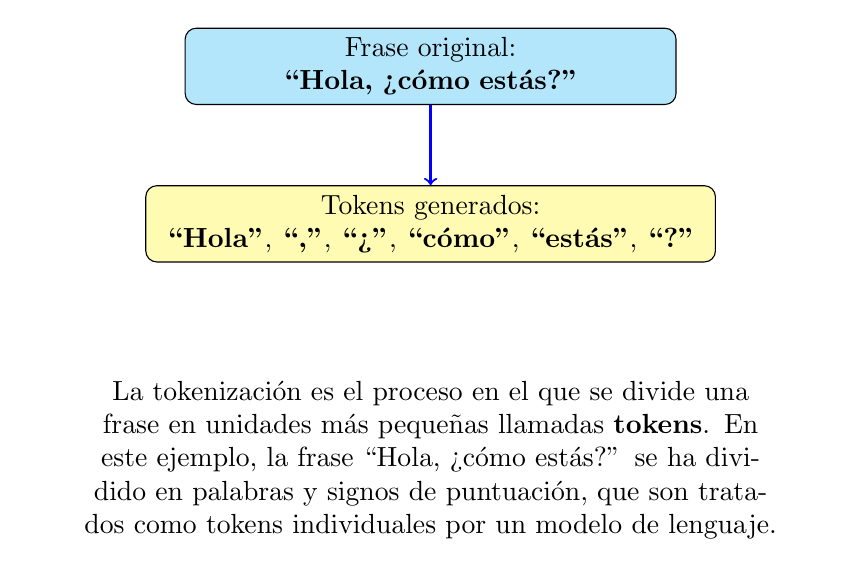
\begin{tikzpicture}[node distance=2cm]

    % Nodo para la frase original
    \node (phrase) [draw, rectangle, fill=cyan!30, text width=6cm, align=center, rounded corners] 
    {Frase original: \\ \textbf{``Hola, ¿cómo estás?''}};
    
    % Nodo para los tokens generados
    \node (tokens) [below of=phrase, draw, rectangle, fill=yellow!30, text width=7cm, align=center, rounded corners] 
    {Tokens generados: \\ \textbf{``Hola''}, \textbf{``,''}, \textbf{``¿''}, \textbf{``cómo''}, \textbf{``estás''}, \textbf{``?''}};
    
    % Conectar nodos con una flecha
    \draw[->, thick, blue] (phrase) -- (tokens);
    
    % Añadir un nodo de explicación
    \node (explanation) [below of=tokens, node distance=3cm, text width=10cm, align=center] 
    {La tokenización es el proceso en el que se divide una frase en unidades más pequeñas llamadas \textbf{tokens}. 
    En este ejemplo, la frase ``Hola, ¿cómo estás?'' se ha dividido en palabras y signos de puntuación, 
    que son tratados como tokens individuales por un modelo de lenguaje.};

\end{tikzpicture}

\subsection{El Cobro por Token}\label{el-cobro-por-token}
Los proveedores de IA, como OpenAI, cobran según la cantidad de tokens utilizados en una interacción. Esto incluye tanto los \textbf{tokens de entrada} (el texto que se envía al modelo) como los \textbf{tokens de salida} (la respuesta generada por el modelo). Este método de cobro es escalable y flexible, lo que lo hace adecuado para empresas de distintos tamaños.

\subsection{Ventajas del Cobro por Tokens}\label{ventajas-del-cobro-por-tokens}
\begin{itemize}
    \item \textbf{Escalabilidad:} Las empresas pueden empezar con un uso pequeño y aumentar conforme lo necesiten.
    \item \textbf{Eficiencia:} Se paga únicamente por el procesamiento real de los datos.
    \item \textbf{Previsión de costos:} Los costos son predecibles, ya que dependen del número de tokens generados en cada interacción.
\end{itemize}

\subsection{Retos del Cobro por Tokens}\label{retos-del-cobro-por-tokens}
Aunque el cobro por tokens es eficiente, también presenta algunos desafíos:
\begin{itemize}
    \item \textbf{Costos acumulativos:} En aplicaciones que requieren grandes volúmenes de datos o respuestas extensas, el costo puede aumentar rápidamente.
    \item \textbf{Dificultad para estimar los costos exactos:} Predecir la cantidad de tokens que generará una interacción puede ser complicado, lo que hace que algunos proyectos subestimen los costos.
\end{itemize}

\subsection{Cómo Optimizar el Uso de Tokens}\label{como-optimizar-uso-tokens}
Para reducir costos y maximizar la eficiencia al trabajar con tokens, se pueden seguir algunas estrategias:
\begin{itemize}
    \item \textbf{Formular preguntas concisas:} Preguntas cortas y precisas generan menos tokens.
    \item \textbf{Limitar el tamaño de las respuestas:} Algunas plataformas permiten establecer un límite de tokens en las respuestas generadas.
    \item \textbf{Agrupar preguntas:} En lugar de realizar múltiples interacciones, es más eficiente agrupar preguntas similares en una sola consulta.
\end{itemize}

\section{APIs para Modelos de Lenguaje Extensos (LLMs)}\label{apis-para-llms}

\subsection{¿Qué es una API en el Contexto de los LLMs?}\label{que-es-api-llms}
Una \textbf{API} permite a una aplicación interactuar con un modelo de IA enviando solicitudes a través de internet. El modelo procesa los datos y devuelve una respuesta. Las APIs de LLMs permiten aprovechar el poder de estos modelos sin la necesidad de entrenarlos desde cero, lo cual reduce costos y tiempos de implementación.

\subsection{Ejemplo Práctico de Uso de API en la Maquiladora}\label{ejemplo-uso-api-maquiladora}
Imagina que tienes una maquiladora de productos electrónicos y deseas optimizar el mantenimiento de las máquinas. Usando una API de GPT, puedes enviar datos históricos sobre fallos de las máquinas y recibir recomendaciones sobre cuándo realizar el mantenimiento preventivo.

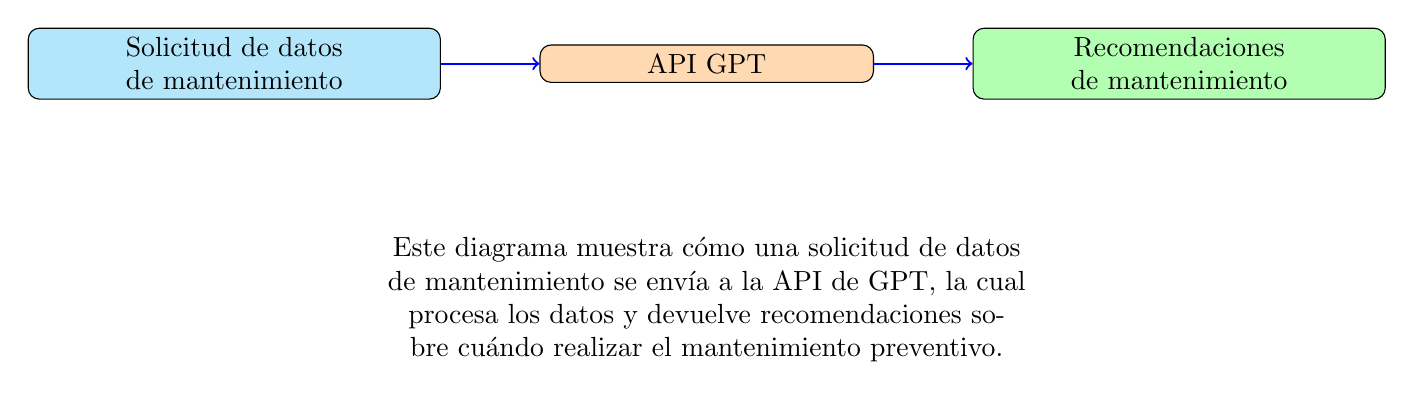
\begin{tikzpicture}[node distance=3cm]

    % Nodo para la solicitud de datos de mantenimiento
    \node (request) [draw, rectangle, fill=cyan!30, text width=5cm, align=center, rounded corners] 
    {Solicitud de datos de mantenimiento};

    % Nodo para la API de GPT
    \node (api) [right of=request, draw, rectangle, fill=orange!30, text width=4cm, align=center, rounded corners, xshift=3cm] 
    {API GPT};

    % Nodo para la respuesta generada
    \node (response) [right of=api, draw, rectangle, fill=green!30, text width=5cm, align=center, rounded corners, xshift=3cm] 
    {Recomendaciones de mantenimiento};

    % Conectar los nodos con flechas
    \draw[->, thick, blue] (request) -- (api);
    \draw[->, thick, blue] (api) -- (response);
    
    % Añadir un nodo de explicación
    \node (explanation) [below of=api, node distance=3cm, text width=10cm, align=center] 
    {Este diagrama muestra cómo una solicitud de datos de mantenimiento se envía a la API de GPT, 
    la cual procesa los datos y devuelve recomendaciones sobre cuándo realizar el mantenimiento preventivo.};

\end{tikzpicture}

\subsection{¿Dónde Encajan los Datos de mi Organización?}\label{donde-encajan-los-datos}

Uno de los primeros pasos para aprovechar la \textbf{inteligencia artificial (IA)} en una maquiladora es entender los tipos de datos que posee y cómo pueden utilizarse. Dependiendo de si los datos son estructurados o no estructurados, se pueden aplicar diferentes enfoques de IA, como \textbf{Machine Learning (ML)} o \textbf{Modelos de Lenguaje Extensos (LLMs)}.

\section{Modelos de Lenguaje Extensos (LLMs) como Primer Paso hacia el Uso de IA}\label{llms-primer-paso-ia}

Aunque los datos estructurados suelen encajar mejor con los algoritmos tradicionales de \textbf{Machine Learning (ML)}, los \textbf{Modelos de Lenguaje Extensos (LLMs)} pueden ser una excelente manera de comenzar a implementar inteligencia artificial en una maquiladora u otro entorno industrial.

Los LLMs, como \textbf{GPT-4} y \textbf{Gemini}, son herramientas poderosas que pueden interpretar grandes cantidades de texto no estructurado, como informes, correos electrónicos, y descripciones de problemas, lo que les permite ofrecer soluciones inmediatas o primeros pasos hacia la automatización.

\subsection{LLMs como Complemento al Machine Learning}
Si bien los algoritmos de ML tradicionales se enfocan en trabajar con datos numéricos estructurados (como métricas de producción, tiempos de ciclo o datos de sensores), los LLMs pueden ser útiles en el análisis de datos textuales no estructurados o en la generación de recomendaciones iniciales. Por ejemplo, en una maquiladora, los LLMs pueden analizar reportes de mantenimiento o de calidad para identificar patrones clave que, más adelante, podrían ser utilizados en modelos tradicionales de ML.

Además, los LLMs pueden interactuar con los datos de manera conversacional, lo que facilita su adopción en los primeros pasos de implementación de IA. Esto permite que los empleados, sin necesidad de conocimientos técnicos profundos, comiencen a beneficiarse de la IA a través de interfaces más accesibles.

\subsection{Comparación de Precisión: LLMs vs Algoritmos de Machine Learning}
Aunque los LLMs tienen capacidades impresionantes para manejar lenguaje natural, en el contexto de predicciones numéricas o análisis basados en datos estructurados, su precisión puede ser algo menor en comparación con los algoritmos tradicionales de \textbf{Machine Learning}. A continuación, se muestra una tabla que compara la precisión promedio de los LLMs frente a algoritmos tradicionales de ML.

\begin{table}[htbp]
\centering
\caption{Comparación de precisión entre Modelos de Lenguaje Extensos (LLMs) y algoritmos tradicionales de Machine Learning (ML) en tareas comunes.}
\label{tab:precision-llm-ml}
\begin{tabularx}{\textwidth}{|X|X|X|}
\hline
\textbf{Tipo de Algoritmo} & \textbf{Modelo/Algoritmo} & \textbf{Precisión Promedio (\%)} \\
\hline
\textbf{Modelos de Lenguaje Extensos (LLMs)} & GPT-4, Gemini, otros modelos generativos & 65-73\% en predicciones numéricas o tareas de análisis de datos estructurados \\
\hline
\textbf{Algoritmos Tradicionales de Machine Learning} & Regresión Lineal, Redes Neuronales, Bosques Aleatorios, SVM & 85-95\% en predicciones numéricas y análisis de datos estructurados \\
\hline
\end{tabularx}
\end{table}

\subsection{Ventajas de Usar LLMs en el Primer Paso hacia la IA}
Los LLMs pueden ser una excelente opción para comenzar a integrar IA en una organización debido a las siguientes ventajas:
\begin{itemize}
    \item \textbf{Accesibilidad:} Los LLMs permiten a los usuarios interactuar con la IA mediante lenguaje natural, lo que reduce la barrera de entrada para su uso.
    \item \textbf{Flexibilidad:} Pueden manejar una amplia variedad de datos textuales no estructurados, como reportes, correos electrónicos y descripciones técnicas.
    \item \textbf{Rapidez en implementación:} Es más rápido implementar LLMs para análisis iniciales, lo que permite obtener valor de los datos sin tener que estructurarlos completamente desde el principio.
\end{itemize}

\subsection{Limitaciones de los LLMs en comparación con Machine Learning}
A pesar de sus ventajas, los LLMs presentan algunas limitaciones cuando se comparan con los algoritmos tradicionales de ML:
\begin{itemize}
    \item \textbf{Menor precisión en tareas numéricas:} Como se muestra en la Tabla \ref{tab:precision-llm-ml}, los LLMs tienen una precisión menor al analizar datos estructurados o numéricos.
    \item \textbf{No son ideales para predicciones complejas basadas en datos históricos:} Los algoritmos de ML, como las redes neuronales y los bosques aleatorios, siguen siendo más adecuados para análisis predictivos complejos.
    \item \textbf{Requieren mayor capacidad computacional:} Aunque los LLMs son poderosos, su costo computacional es generalmente mayor que el de los modelos tradicionales de ML.
\end{itemize}

\subsection{Conclusión: LLMs como Puerta de Entrada a la IA}
En resumen, los LLMs pueden ser una herramienta poderosa para que las organizaciones comiencen su viaje hacia la automatización inteligente. Aunque no alcanzan la misma precisión que los algoritmos tradicionales de Machine Learning en ciertos tipos de tareas, su capacidad para interactuar con datos no estructurados y su accesibilidad los convierten en una opción ideal para dar los primeros pasos en la implementación de IA.

``Los LLMs son la puerta de entrada hacia el mundo del Machine Learning, proporcionando un puente accesible entre la interacción humana y la automatización avanzada.''

\section{¿Dónde Encajan los Datos de mi Organización?}\label{donde-encajan-los-datos}

Uno de los primeros pasos para aprovechar la \textbf{inteligencia artificial (IA)} en una maquiladora es entender los tipos de datos que posee y cómo pueden utilizarse. Dependiendo de si los datos son estructurados o no estructurados, se pueden aplicar diferentes enfoques de IA, como \textbf{Machine Learning (ML)} o \textbf{Modelos de Lenguaje Extensos (LLMs)}.

\begin{table}[htbp]
\centering
\caption{Ejemplos de tipos de datos en una maquiladora y aplicaciones de Machine Learning (ML) y Modelos de Lenguaje Extensos (LLMs).}
\begin{tabularx}{\textwidth}{|X|X|X|X|}
\hline
\textbf{Tipo de Datos} & \textbf{Descripción} & \textbf{Modelo Adecuado} & \textbf{Ejemplo de Aplicación} \\
\hline
Numéricos estructurados & Datos organizados en tablas o bases de datos, como registros de producción diaria, tiempos de ciclo, consumo de energía. & Machine Learning (ML) & Predicción de fallos de máquinas, optimización de inventario, análisis de tiempos de ciclo. \\
\hline
Texto no estructurado & Informes de mantenimiento, correos electrónicos, descripciones de problemas técnicos. & Modelos de Lenguaje Extensos (LLM) & Análisis de reportes de fallos, generación automática de resúmenes, asistente virtual para consultas sobre mantenimiento. \\
\hline
Imágenes & Fotografías capturadas por cámaras de control de calidad en las líneas de producción para detectar defectos. & Machine Learning (ML) & Detección de defectos mediante visión por computadora, inspección de calidad automatizada. \\
\hline
Datos de sensores (IoT) & Sensores conectados a máquinas, como temperatura, vibración, velocidad de operación. & Machine Learning (ML) & Mantenimiento predictivo, monitoreo en tiempo real, optimización de eficiencia energética. \\
\hline
Datos de PLC (Programmable Logic Controller) & Datos generados por controladores lógicos programables, como ciclos de máquina y activación de actuadores. & Machine Learning (ML) & Optimización de la programación del PLC, detección de patrones anormales, mantenimiento predictivo. \\
\hline
Datos SMT (Surface-Mount Technology) & Registros de colocación de componentes, tiempos de ciclo, análisis de defectos de ensamblaje en productos electrónicos. & Machine Learning (ML) & Optimización de líneas SMT, reducción de scrap, análisis de defectos en fabricación electrónica. \\
\hline
Datos médicos ocupacionales & Información sobre la salud de los trabajadores, como ritmo cardíaco y niveles de estrés en tiempo real. & Machine Learning (ML) & Prevención de riesgos laborales, monitoreo de salud en tiempo real, optimización de turnos según fatiga. \\
\hline
Datos de seguridad laboral & Registros de accidentes laborales, incumplimientos de normas, condiciones ambientales peligrosas. & Machine Learning (ML) & Prevención de accidentes mediante análisis predictivo, alertas automáticas de condiciones peligrosas. \\
\hline
Datos de control de calidad & Métricas de calidad y pruebas de resistencia o durabilidad, tanto destructivas como no destructivas. & Machine Learning (ML) & Análisis predictivo de calidad, optimización de procesos de inspección, ajuste de parámetros en tiempo real. \\
\hline
Datos energéticos & Medición de consumo de energía por máquinas y líneas de producción. & Machine Learning (ML) & Optimización del consumo energético, predicción de picos de consumo, reducción de costos energéticos. \\
\hline
\end{tabularx}
\label{tab:responsive-table}
\end{table}

\section{Modelos de Lenguaje Extensos (LLMs) como Primer Paso hacia el Uso de IA}\label{llms-primer-paso-ia}

Aunque los datos estructurados suelen encajar mejor con los algoritmos tradicionales de \textbf{Machine Learning (ML)}, los \textbf{Modelos de Lenguaje Extensos (LLMs)} pueden ser una excelente manera de comenzar a implementar inteligencia artificial en una maquiladora u otro entorno industrial.

Los LLMs, como \textbf{GPT-4} y \textbf{Gemini}, son herramientas poderosas que pueden interpretar grandes cantidades de texto no estructurado, como informes, correos electrónicos, y descripciones de problemas, lo que les permite ofrecer soluciones inmediatas o primeros pasos hacia la automatización.

\subsection{LLMs como Complemento al Machine Learning}
Si bien los algoritmos de ML tradicionales se enfocan en trabajar con datos numéricos estructurados (como métricas de producción, tiempos de ciclo o datos de sensores), los LLMs pueden ser útiles en el análisis de datos textuales no estructurados o en la generación de recomendaciones iniciales. Por ejemplo, en una maquiladora, los LLMs pueden analizar reportes de mantenimiento o de calidad para identificar patrones clave que, más adelante, podrían ser utilizados en modelos tradicionales de ML.

Además, los LLMs pueden interactuar con los datos de manera conversacional, lo que facilita su adopción en los primeros pasos de implementación de IA. Esto permite que los empleados, sin necesidad de conocimientos técnicos profundos, comiencen a beneficiarse de la IA a través de interfaces más accesibles.

\subsection{Comparación de Precisión: LLMs vs Algoritmos de Machine Learning}
Aunque los LLMs tienen capacidades impresionantes para manejar lenguaje natural, en el contexto de predicciones numéricas o análisis basados en datos estructurados, su precisión puede ser algo menor en comparación con los algoritmos tradicionales de \textbf{Machine Learning}. A continuación, se muestra una tabla que compara la precisión promedio de los LLMs frente a algoritmos tradicionales de ML.

\begin{table}[htbp]
\centering
\caption{Comparación de precisión entre Modelos de Lenguaje Extensos (LLMs) y algoritmos tradicionales de Machine Learning (ML) en tareas comunes.}
\label{tab:precision-llm-ml}
\begin{tabularx}{\textwidth}{|X|X|X|}
\hline
\textbf{Tipo de Algoritmo} & \textbf{Modelo/Algoritmo} & \textbf{Precisión Promedio (\%)} \\
\hline
\textbf{Modelos de Lenguaje Extensos (LLMs)} & GPT-4, Gemini, otros modelos generativos & 65-73\% en predicciones numéricas o tareas de análisis de datos estructurados \\
\hline
\textbf{Algoritmos Tradicionales de Machine Learning} & Regresión Lineal, Redes Neuronales, Bosques Aleatorios, SVM & 85-95\% en predicciones numéricas y análisis de datos estructurados \\
\hline
\end{tabularx}
\end{table}

\subsection{Ventajas de Usar LLMs en el Primer Paso hacia la IA}
Los LLMs pueden ser una excelente opción para comenzar a integrar IA en una organización debido a las siguientes ventajas:
\begin{itemize}
    \item \textbf{Accesibilidad:} Los LLMs permiten a los usuarios interactuar con la IA mediante lenguaje natural, lo que reduce la barrera de entrada para su uso.
    \item \textbf{Flexibilidad:} Pueden manejar una amplia variedad de datos textuales no estructurados, como reportes, correos electrónicos y descripciones técnicas.
    \item \textbf{Rapidez en implementación:} Es más rápido implementar LLMs para análisis iniciales, lo que permite obtener valor de los datos sin tener que estructurarlos completamente desde el principio.
\end{itemize}

\subsection{Limitaciones de los LLMs en comparación con Machine Learning}
A pesar de sus ventajas, los LLMs presentan algunas limitaciones cuando se comparan con los algoritmos tradicionales de ML:
\begin{itemize}
    \item \textbf{Menor precisión en tareas numéricas:} Como se muestra en la Tabla \ref{tab:precision-llm-ml}, los LLMs tienen una precisión menor al analizar datos estructurados o numéricos.
    \item \textbf{No son ideales para predicciones complejas basadas en datos históricos:} Los algoritmos de ML, como las redes neuronales y los bosques aleatorios, siguen siendo más adecuados para análisis predictivos complejos.
    \item \textbf{Requieren mayor capacidad computacional:} Aunque los LLMs son poderosos, su costo computacional es generalmente mayor que el de los modelos tradicionales de ML.
\end{itemize}

\subsection{Conclusión: LLMs como Puerta de Entrada a la IA}
En resumen, los LLMs pueden ser una herramienta poderosa para que las organizaciones comiencen su viaje hacia la automatización inteligente. Aunque no alcanzan la misma precisión que los algoritmos tradicionales de Machine Learning en ciertos tipos de tareas, su capacidad para interactuar con datos no estructurados y su accesibilidad los convierten en una opción ideal para dar los primeros pasos en la implementación de IA.

``Los LLMs son la puerta de entrada hacia el mundo del Machine Learning, proporcionando un puente accesible entre la interacción humana y la automatización avanzada.''
